
\status{Mostly written}

\plan{Explain why we want $P$ engines when there are $P$ processors}
As explained in Chapter \ref{chap:background} Mercury manages its parallel
work with userspace scheduling.
Parallel tasks are represented by contexts or sparks,
depending on whether the task has started execution or not.
Engines run contexts and can switch between them without using the operating
system.
We use a set of operating system threads,
each thread running a Mercury engine.
The operating system manages these threads including their mapping onto
processors.
The number of engines, and therefore threads, to use is configurable.
In order to make use of each of the system's processors we should create at
least one thread for each processor.
However creating more than one thread per processor consumes more resources
than we need,
and if more than one thread is actively using the same processor the
operating system must perform context switches between these threads.
Therefore the runtime system by default uses the same number of engines as
there are processors in the system.
\plan{Explain briefly how we detect how many processors there are,}
We have been using the \code{sysconf} system call to detect the number of
processors in the system.
This is supported on a number of platforms but support is not guaranteed to
exist.
If Mercury cannot detect the number of processors in the system it will
use a single engine.

\plan{Explain why we want thread pinning.}
We have been relying on the operating system to assign threads onto
processors,
this is usually acceptable but it is generally considered more reliable to
pin threads to specific processors.
This is beginning to become more important as processors are made with
larger numbers of cores and therefore more complex memory hierarchies.
\plan{Explain how we get thread pinning.}
We can \emph{pin} a thread to a specific processor using the
\code{setcpuaffiny()} system call,
this call is available on many Unix-like OSs.
Our initial thread pinning implementation pinned each of Mercury's engines
to a separate processor,
ensuring that they are evenly distributed and are not migrated onto new
processors.
Thread pinning can also be used with when the user requests fewer engines
than processors.
When the user requests more engines than processors only the first $P$ are
were pinned (where there are $P$ processors).

\begin{figure}
\begin{center}
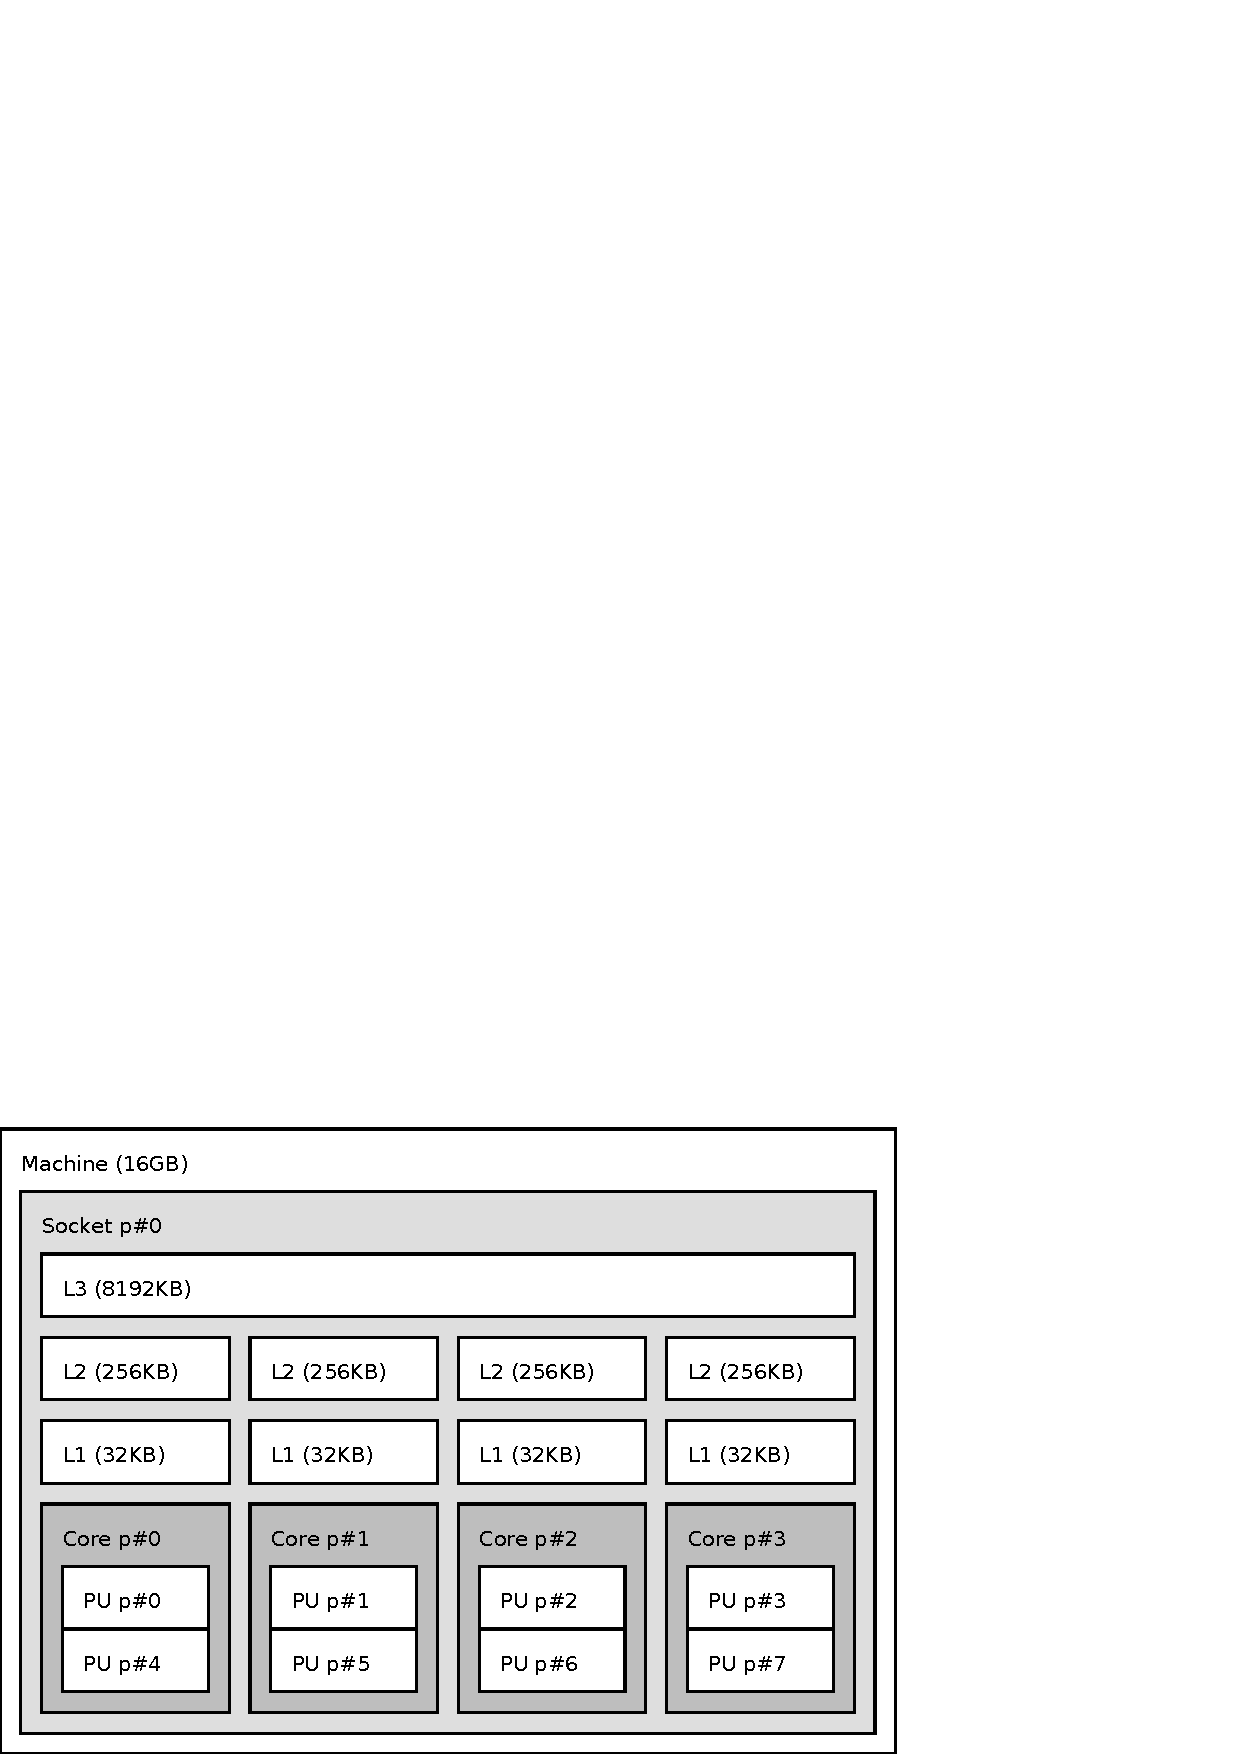
\includegraphics[width=0.75\textwidth]{i7-hierarchy}
\end{center}
\caption{Memory hierarchy of the Intel i7-2600K processor and 16GB of main
memory}
\label{fig:i7_hierarchy}
\end{figure}

\plan{What about SMT, not all processors are equal.}
This works well on many SMP (symmetric multiprocessing) systems.
However, on systems that use SMT\footnote{
    SMT is sometimes called ``hyperthreading'' especially for marketing.}
(symmetric multithreading) as well as SMP this can be problematic.
Consider the memory hierarchy of the Intel i7-2600K processor
(Figure \ref{fig:i7_hierarchy}).
The i7-2600K has four cores, each with two hardware threads (PUs in the
figure).
If Mercury successfully detects that the system has eight logical processors
or the user specifies eight engines then thread pinning will correctly pin
each engine to a separate thread.
However,
if the user requests only four engines, which cores will be used?
depending on how they are selected,
and how the OS's \code{setcpuaffinity()} system call labels them all four
mercury engines could be pinned to just two of the CPU's cores instead of
being distributed uniformly across all four cores.
Uniform distribution will result in higher performance for the Mercury
program,
but it may affect other processes running on the same system.

\plan{How do we handle SMT}
Unfortunately there is no portable method for querying the OS about the
system's memory hierarchy.
Therefore we use the Portable Hardware Locality (hwloc) library
\citep{broquedis:2010:hwloc}.
Hwloc provides some tools such as the one that drew Figure
\ref{fig:i7_hierarchy},
but more importantly it provides an API for querying the memory hierarchy of
the system and methods for pinning threads to (sets of) cores or hardware
threads.
We use hwloc to determine the number of hardware threads in a system,
and optionally pin engines to hardware threads.
If the user specified the number of engines to use then we pin each engine
to a hardware thread in each core so that engines are distributed to cores
as evenly as possible.
If the user specifies more engines than are available
(which we admit would be silly) then we allow more than one engine per
hardware thread,
meanwhile keeping engines as evenly distributed as possible amongst the
threads and cores.

%\paul{I am not going to talk about busy waiting since I have not written the
%runtime system in a way that I can test or change this easily.}

\plan{Benchmarks}

\plan{Further work}
As we discussed in the previous section,
knowledge of the memory hierarchy could help make better scheduling
decisions.
When using thread pinning we can guarantee that a particular engine is
running on a particular processor/hardware thread,
combining this with information about the memory hierarchy such as shared
caches/sockets we can know which processors share the same cache(s) with the
current processor either prefer to steal work from them or send work to
them.

